What exactly is meaning? How does language express it? These are some of the most central questions in the project of creating a language. When creating Atlan, we tried to create a meaningful set of signs, meaningful words that expresses people's intentions. We tried to do this by creating a vocabulary, words were created —better put, generated— with a given, unchanging meaning. However, is that how meaning works? Do not words mean what they mean because other people understand them to mean those things. Meaning is inevitably tied up with use. How can we then create meaningful words before anybody uses them? 

These are very fundamental questions about language, tough questions, and questions that inevitably, Atlan will have to deal with. We went into this project with the belief that meaning of words can be given from above, words have meaning because the dictionary shows they do. In Atlan, to give meaning to signs, we have differentiated between language and speech; separated the linguistic code and the daily utterances. Following a structuralist understanding of language we separated meaning as depending on two things as Ferdinand de Saussure argued (Saussure 1959); language is (1) the linguistic code, this is the structure of grammar\idx{grammar} and syntax\idx{syntax}, the meaning of words as you find them in the dictionary; (2) how people use the language in a certain context and what people \textit{do} with language, i.e. to order something or to begin a conversation (What does “hello” actually mean?) —what the linguist John Austin has called speech acts (Austin 1955)— In linguistics this second facet of meaning in language is the focus of the subdomain pragmatics\idx{pragmatics}. This subdomain hopes to answer how intention, speech and language interact and create meaning and understanding between speakers. This chapter will engage with pragmatics\idx{pragmatics} in the creation of Atlan. 

It is important to engage with Pragmatics\idx{pragmatics} when creating a conlang because, although certain structures in language will indicate certain things grammatically, what speaker does with language is eventually what makes the language a language. A conlang might have a very thorough structure of grammatical rules but how do you use it? Comical examples of conlangs that do not engage with the question of speech are legion, for example Leibniz attempts of a perfect language based on a clear and logical structure in the end became calculus (Eco\idx{Eco, Umberto} 271), a beautiful perfected ‘language’ but nearly impossible to have a conversation in. Also, we must know whether the use of a conlang leads to clear and meaningful understanding and not that there is something of vital importance to that thing we call language that we have overlooked. How meaning in language is expressed, in the end, depends on the speakers, what they intend to do when speaking. Whether that be communicating information or emotion\idx{emotion}al expression.  

We cannot separate meaning from use, otherwise beautiful linguistic phenomena like metaphors, metonymies and curse words would only be false or incorrect. Poetry, only a net of lies and falsehoods. It is clear there is an inherent link between the meaning of language, what linguists call; semantics\idx{semantics}, and the use of language, that is, pragmatics\idx{pragmatics}. As linguists like, for example, Gennaro Chierchia has shown these two facets cannot be understood separate (e.g., Chierchia 2012).  

Atlan, of course, is made with the goal of a language that can function as an international lingua franca. A language to assist speakers of different languages to communicate. It has a very practical goal. However, people never seem to use language as the grammar\idx{grammar}ians want. Besides that, how does Atlan with phenomena like curse words; they depend not only on the semantic meaning but also on whether they {\it sound\idx{sound} right}, express the feeling right. “Holy cow” for example, does not mean what it does semantically, it expresses shock and confusion. In Atlan we might have a way thatto describe how to semantically describe a “holy cow” but how do we express our shock in the same way as in English? Even if we can make the meaning explicit, telling exactly what the feeling is but will that truly express the feeling? Is telling and expressing the same thing? Another problem is that language is never finished, it is made anew by how its speakers use it every day. Every speaker is a language maker, \footnote{Especially the linguistic theories of the iconoclastic linguist Roy Harris focuses on this point} making a new language to express their experiences and not merely to describe them. This is a problem for our ambitions with Atlan because, it will mean a disconnect with the grammatical rules and the daily use, the language that way would soon fall apart, every speaker with its own version. This is what the writer Umberto Eco\idx{Eco, Umberto} in his book about conlang called: “the inescapable Babel\idx{Babel} effect” (Eco\idx{Eco, Umberto} 323), named after the biblical story of the tower of Babel\idx{Babel}. In the story humans in the beginning speak only one language and build a tower as a monument to themselves. However, soon they find that their speech is confused with each having a differ way of speaking. The inescapable Babel\idx{Babel} effect is the seemingly unavoidable confusion that is a result of people using language in their own way. This effect puts a wrench on our ambitions with Atlan. The only thing we can do with this project is to create a linguistic structure that, if it was used correctly, would lead to easy and clear communication between speakers. The conlang searches for a perfect \textit{prescriptive} linguistic code. It cannot control how people really use it, the conlang cannot create perfect speech. Pragmatics\idx{pragmatics} cannot be prescribed; it cannot be perfected; it is about how people \textit{use} language not about how people \textit{ought to} use language.  

However, what we can do is to build implicit meanings into the semantics\idx{semantics} of Atlan to make the language as clear as possible no matter how people use it. To do this Atlan makes explicit what the intention is of the sentence, as far as this is possible. This chapter, on the one hand, will look at a linguistic theory about intention and speech. Afterwards it will look at how language changes depending on its use. How language relates to culture and its speakers. Whether Atlan can escape the Babel\idx{Babel} effect. I will finish with a synopsis of how language should be understood and if Atlan can be used practically.  

\vspace{-0.5cm}
\section{Implicatures}

In linguistics the term implicature means the implicit intention that a speaker has with an utterance. (Davis 2016) An implicature being what the speaker intends to do or say when speaking. In luigistics this term is usefull for it describes the meaning that a speaker puts into a word. How meaning in language is achieved depends on what the speakers implicature is with an utterance.

\subsection{Prosody\idx{prosody}}

In natural language the non-explicit markers of speech like word-stress or rhythm might be used to indicate what the intention is behind an utterance (Wichmann 2009). This is called prosody\idx{prosody}; intonations, stress and rhythm that mark intentions of the speaker and can carry meaning or information. However, in Atlan the decision has been made that prosodic markers should have no semantic or pragmatic value\footnote{For more on this topic Niek’s chapter will suffice.} . Although, this is not completely true, Atlan still uses stress markers, but prosodic markers, are for the most part meaningless. Regardless to avoid confusion and ambiguity meaning that in English are not grammatical but based on prosodic markers are in Atlan grammatically marked. The five vowel syllable\idx{syllable}s are used for these effects:

\begin{itemize}
{\small
\item[\kern-0.4em\Atlano]   $\approx$ o = Exclamative (prosody\idx{prosody}), imperative, vocative 

\item[\Atlane]  $\approx$ e =Interrogative (question, prosody\idx{prosody}\footnotemark)    
	\footnotetext{The letter {\it e}\/ can also be used as a so-called 'filler word', like 'uhmm' or 'ehmm'}

\item[\Atlana]   $\approx$ a + stress = Stress marker (prosody\idx{prosody}) 

\item[\kern0.4em\Atlani]   $\approx$ i (+ pronoun) = Relative clause   

\item[\Atlanu]   $\approx$ u  = Subjunctive (wish)
	}
\end{itemize}

\noindent The Atlan vowel that is most like the English vowel “a” is a stress marker, indicating that the word is important for the \textit{implicature} of the sentence. The equivalent in English script would be to write a word in italics. (Take the difference between the sentence “Are you going to \textit{the cinema?”} and “\textit{Are} you going to the cinema?” the first questioning the location and the second questioning if the it is true or not that you are going to the cinema.) because italics is impossible in the Atlan script an extra sign will be needed, likewise in the spoken language is the stress marker already used to indicate the core of the word and thus a vowel marker can be used to for fill the same function that stress has in a language like English.  

What these prosody\idx{prosody} markers show is that when speaking the message is more than just the sum of the words. Every utterance has implicit information that the listener can only understand by placing it in the context of the conversation or by non-linguistic signs like laughter and body language. How Atlan speakers communicate the information that in a natural language like English would be done with prosody\idx{prosody} is though the grammar\idx{grammar} of the language. However, to communicate does not necessarily mean you are using language (It might also be said that using language does not necessarily mean you are communicating). By using these explicit markers Atlan can help its speakers to make their intentions clear in a way that would otherwise be impossible or ambiguous. 

\vspace{-0.2cm}
\subsection{Intentions in speech}

As we have seen, Atlan incorporates much of the intention of a speaker into the grammar\idx{grammar}, making explicit what in many natural languages was implicit. (This is not to say that these markers are not seen in natural languages Greek for example does have a stress marker “$\gamma\epsilon$” similar to Atlan’s \Atlana ≈ a (Liddell 1894:301)) Yet it is simply not possible nor desirable to make every meaning that a word might carry explicit into the grammar\idx{grammar}. Atlan is a language; it needs to be interpretated; not decoded.

Implicatures, by definition, cannot be incorporated into the semantic structure. Nevertheless, a language needs to make it crystal clear what is meant with an utterance. Ambiguity of meaning is something we are attempting to avoid. However, what a speaker might intend to say is manifold. What we have done with Atlan is to divide the possible intention within speech into different uses of language. This way we can make sure that all the possible intentions of an utterance can be expressed in Atlan. The classification is based on the understanding of language of the linguist and literary theorist Roman Jakobson. In Jakobson's theory the meaning of speech depends on six possible uses that an utterance might have, based on six factors that are the most important in understanding speech. These factors are: (1) the speaker (ADDRESSER), (2) the listener (ADDRESSEE), the utterance that caries (3) a MESSAGE, (4) a CONTEXT in which it is uttered, whether there is (5) CONTACT between the listener and speaker and (6) the linguistic CODE, meaning the grammar\idx{grammar} and lexicon the interlocuters both understand. These factors can be visualised like this:

\small
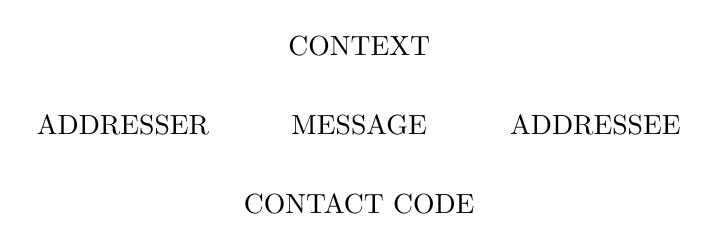
\begin{tikzpicture}
\node(A) at (0,1){ADDRESSER};
\node(B) at (3,0){CONTACT CODE};
\node(C) at (3,1){MESSAGE};
\node(D) at (3,2){CONTEXT};
\node(E) at (6,1){ADDRESSEE};
\end{tikzpicture}
\normalsize

\vspace{-.1cm}
{\it \footnotesize Figure 1: Jakobson's factors of meaning in speech (Jakobson, 2018, p.1070)}
\vspace{0.3cm}

\noindent In every utterance all six factors are present. However, interpretating which factor has the most importance is how the recipient understands the intention of the utterance. Connecting the function with the most important factors we get a schema of the six different ways to use language: 

\vspace{0.3cm}

\small
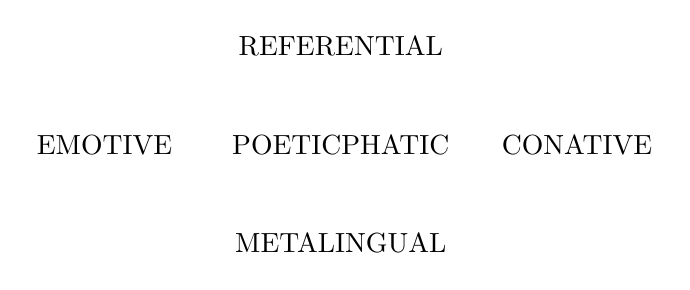
\begin{tikzpicture}
\node(A) at (0,1.25){EMOTIVE};
\node(B) at (3,0){METALINGUAL};
\node(C) at (3,1.25){POETIC \\ PHATIC};
\node(D) at (3,2.5){REFERENTIAL};
\node(E) at (6,1.25){CONATIVE};
\end{tikzpicture}

{\it \footnotesize Figure 2: Six different uses of language (Jakobson,2018, p.1074)}

\vspace{0.3cm}


When the most important factor is the addresser (so the person speaking), the intention behind an utterance becomes \textit{emotive}; that means that what the speaker is feeling or thinking is most important to communicate. Take, for example, the sentence: “It is raining"\footnote{These examples are found  in the lecture on Jakobson by Paul Fry (Fry 2009).}. When the intention is to use this sentence in an emotive way “It is raining” is a dramatic metaphor like one might find in a romantic poem. An expression of sadness and gloom ‘it is raining in my soul.’ The reader or listener must understand this sentence as expressing what the speaker is feeling. 						

When the factor of the addressee becomes central the \textit{conative} function is most important. This is when the utterance becomes an implicit command, for example a mother seeing her child go outside without a jacket might say “It is raining” meaning a command to put a jacket on. 				
When the utterance is focused on the \textit{context} around  the speakers the function becomes referential. This is when the weatherman says, “It is raining,” merely saying the factual state of the nature around  the speakers. 				

When an utterance is intendent to establish contact (the “Do you hear me?” and “Hello” of language) the function of the speech is \textit{phatic}. Take for example the scene of two awkward young people on a date, both are awkwardly silent and then one of them says “oh, it is raining.” the speaker does not actually care whether it is raining or not, the utterance is simply meant to establish contact. 						
The \textit{metalingual} function is the ability of language to talk about itself. It is Language to correct and explain language. Like how I have been using the sentence “It is raining.” for example but also, questions like ‘what do you mean with “it” when you say, “it is raining?”’ (Actually, a very puzzling question) 							

Lastly there is the \textit{poetic} function, the function that targets the message of an utterance. This might mean the form and rhythm of an utterance or the combination of different concepts in witty similarities. A good example our supervisor Ana gave is: “it is raining bullets.” What is important in the poetic function is the relation between speech and message, the utterance is calling attention to the how and why language works\footnotemark. Instead of selecting the proper word a speaker combines words. Similar to the metalingual function the poetic function focuses of language as a semiotic system. However, the poetic function and metalingual function are in diametrical opposition to each other; the metalanguage function is about how the sequence of words is used to build an equation (‘rain means falling water’ for example) whereas in the poetic function the equation is used to build a sequence (‘look how the shape of the drops of rain resemble bullets’)\footnote{Jakobson explains this with the difficult sentence of : “The poetic function projects the principle of equivalence from the axis of selection into the axis of combination.” (Jakobson 2018:1074)}.

\footnotetext{It is interesting to note that, because every possible syllable in Atlan has a designated meaning associated with it, creating rhyming poetry might be surprisingly easy, because each syllable will rhyme with at least a few others.}

These are the six functions that language has. One way we might get a crystal-clear language is by having the speaker explicitly state that an utterance has one of these six functions. Having a marker to indicate the function. However, besides being very inelegant, that would lead to ridiculous sentences. Besides that, it is an international auxiliary language and was never intended to replace natural languages, merely to work as a tool to easily communicate with speakers with different mother tongues. These functions in language are unavoidable but the aim of Atlan is to make a language that is semantically unambiguous and simple. Atlan, as it is now, is a language whose makeup is heavily tilted to utterances that referent the world as it presents itself for it creates words based on the speaker's empirical data of the world. How people can understand each other in Atlan is though understanding the words as collections of basic axioms, axioms that are experienced in the world. To say “it is raining” in the emotive sense in Atlan you would be better off by arriving to that emotion\idx{emotion} by the emotive axioms of Atlan. Saying “it is raining” in all the different ways as described above clashes with the aim to counter ambiguity in the language. You have to say what you mean to be able to form the words of Atlan. Thus, the language, in the way it forms its words, is always referencing the experience that such a concept entails.   

\section{Culture and Language}


As Max’s introduction already discussed it is difficult to separate culture and worldview from language. Nevertheless, with Atlan we are attempting to do exactly that, in the name of a neutral language. In relation to culture Atlan set out to achieve two things: (1) Atlan needed to be independent to any dominant culture, otherwise it would be no better than English as a neutral lingua franca; (2) cultural expression and lived world needed to be able to be translated into and even be able to be expressed in Atlan. As Max also discussed the relation between language, country, politics and worldview is a very contentious topic and a cause for problems in any auxiliary language. On the one hand, Atlan will need to engage with expression within a specific cultural milieu. But on the other hand, Atlan hopes to be able to evade being tied up to any specific cultural expression as much as that is possible.				 		

We consciously made Atlan as culturally neutral as we could and hoped to give the language enough scope to be able to express all kinds of different worldviews and culturally specific practices and items. It is after all a language that hopes to bridge linguistic and nationalistic divides, this means that it needs to make different culturally specific expression understandable to all speakers. As we have discussed in 7.1previous part Atlan is a language that should focus on the referential use of language. It is a language that tells you the facts as they are for the speaker. This might limit the speaker's cultural expression of the world. What is more important is that people can understand each other, even if that would limit their expressive ability. Here we see why culture is impossible to separate from language; already in Atlan there is a hierarchy of values; comprehension is more important than expressions. 					 

Language without culture is an impossibility and the worldview of its speakers, if language has influence on that, will still be influenced by Atlan just like any other language would do. How Atlan changes its speaker's way of life is evident by its very concept as auxiliary language. To use an auxiliary language a speaker must be open to other cultures and other ways of speaking, especially in our language Atlan. The phonetic of Atlan is such that its speakers need to broaden theirthere understanding of a specific sound\idx{sound} more than their mother tongs would most likely do. Atlan speakers need to be very open and conscientious because words have many ways of being expressed and a concept might be expressed in many different ways. 									 

Consequently, even though Atlan tries to separate language and the sociolinguistic context, it is very questionable that such a thing can be achieved. As the linguist Alvino Fantini argued language and speakers' values, beliefs and attitudes are mutually interdependent. (Fantini 2020) The symbols that make up a language can only be understood in a sociolinguistic context and are interrelated with the worldview and norms, values and beliefs of the speaker. (Fantini 2020:270)		

It is inevitable that Atlan will create its own sociolinguistic context. We might then question whether Atlan is an improvement to a natural language like English as lingua franca. Afterall we had rejected English because it relates to one particular culture and not with all cultures and now it seems that Atlan will only create a new singular milieu: “Two things seem to happen simultaneously: people attempt to fit their language to a situation or context that their language, in turn, helped to create in the first place (Gee qtd. in Kecskes 2008:146).”  				 

This is a problem for Atlan however, it we hope to avoid this problem by making Atlan a very open and lose language. For example, with the phonemes being very flexible and not really having one correct way to say a word. We hope that this creates a culture around  Atlan that is similar to a bilingual or multilingual interaction. What is called by Fantini ‘incipient’ behaviour: 

\begin{quote} 

Simply put, this stresses an attitude of willingness to 	engage with others with no common tongue (not an		uncommon situation) and attempting to communicate. In 	this view, bilingualism begins with attitude, with a 		willingness to engage, even when no skill exists.	(Fantini 273)  

\end{quote} 

Atlan would hopefully create a loose social linguistic milieu that makes it more likely for people from different ethnicities and cultures to try and understand each other. More than if the language would be a natural language like English because in English there is less space for different ways to say something. However, this openness might also be problematic because of the “inescapable Babel\idx{Babel} effect” that we discussed in the introduction of this chapter. More language variation\idx{language variation} will create more confusion. Atlan does not avoid the Babel\idx{Babel} effect, on the contrary, it amplifies it.

\section{Is language grammar\idx{grammar}?}

So far, we have looked at pragmatics\idx{pragmatics} as a source of problems for Atlan. Whether Atlan can express all the functions of language, how pragmatic use confuses Atlan into incomprehensibility, whether orit is not it is impossible to separate language from culture and, lastly, whether language is only meaningful in a sociolinguistic milieu. The pragmatic use of language has been an obstacle to be overcome. The focus was to make a grammatical structure without ambiguities, easy to understand and simple in structure, yet when faced with the task of speaking Atlan it quickly becomes unwieldy and confusing.			 

What my colleagues and I hopedset out to achieve was to create a perfect language first and then see whether people can use it.  We started with the grammar\idx{grammar} and machine algorithms and from there moved on to use. Leaving pragmatics\idx{pragmatics} for the end of the book. It is reasonable to wonder whether this is the best way to understand language. Does language exist without speakers using it? Do the rules of language form the basis for speech or does speech form the basis for the rules of language? The linguist Roy Harris attacks the notion of grammar\idx{grammar} as the basis of language. For him, to understand language, you must place speech/ use first.first. (Haris 1987) Steven Knapp and Benn Michaels Walter take this even further arguing that there is only intention and words, there is no language without speakers. (Knapp and Walter 1985) In other words, a room full of chimpanzees typing at random on typewriters would never create a work of Shakespeare. It could only create a piece of paper with letters on it that look like a work of Shakespeare. A true work of Shakespeare needs to have the intention of an author behind it to be language. These “neo-pragmatic” thinkers show that it is not obvious that we get to a perfect language (or any language at all for that matter) by creating an abstract grammatical structure. 

Many artists and poets are not so sure of our view on language either. The French poet Mallarmé for example rebelled against the notion that things mean what the dictionary says they mean, putting a lot of emphasis on the emotion\idx{emotion} that the sound\idx{sound} of a word invokes. (The French word Jour for example was for Mallarmé to sombre to express “day” and Nuit to joyful.) The futurist project of Zaum is another example; this Zaum ‘language’ has no grammar\idx{grammar} or syntax\idx{syntax} rules and consists of neologisms. It was created by the Russian avant-Garde poets Aleksei Kruchenykh and Velimir Khlebnikov to show that language doesn't dependend on grammatical rules (Tynyanov 1979).						 

That language has an element of what I can only describe as a feel of the language is nicely exemplified in nonsense poetry. Utterance can create significance and meaning even when they should not like in Lewis Carrol’s Jabberwocky (Carrol qtd. in Hofstadter 366):

\begin{quote}
Twas bryllyg, and the slythy toves 
 Did gyre and gymble in the wabe: 
 All mimsy were the borogoves; 
 And the mome raths outgrabe.  
\end{quote}

\noindent Here Lewis Carrol has created a poem mostly made of non-existent words, yet everybody believes that he or she can understand it. ‘It feels right.’ This is also shown in the numerous translation\idx{translation}s made of the poem that reproduce the nonsense words but then in, among others, a French (Frank L. Warrin qtd. In ibid 366) and German (Robert Scott qtd. In ibid 366) setting: 

\begin{quote}
Il brilgue: les t\^{o}ves lubricilleux 
Se gyrent en vrillant dans la guave. 
Enm\^{i}n\'{e}s sont les gougebosqueux 
Et le m\^{o}merade horsgrave.  

Es brillig war. Die schlichten Toven 
Wirrten un wimmelten in Waben 
Uns aller-m\"{u}msige Burggoven 
Die mohmen R\"{a}th’ ausgraben 
\end{quote}

\noindent How then would we be able to translate this poem and linguistic playfulness into Atlan? We cannot. Atlan is too phoneticly flexible, it does not have one specific correct sound\idx{sound} and its words are not ordered around  associations or ‘family resembles’ like in English or French. Pragmatic linguists have a different approach to language than we had when making Atlan. Their understanding of language is shown in linguistic phenomena that Atlan cannot replicate.   

\section{Conclusion}

To sum up, this chapter discussed the pragmatic use of language and what this would entail for Atlan. It discussed how Atlan makes explicit what in natural languages is only implicit, but Atlan can only go that far in incorporating the intentions of speakers into the grammar\idx{grammar}. Furthermore, the chapter engaged with the worry that Atlan’s loose structure will dissipate and confuse the semantic unity of the conlang and that, while Atlan avoids having a dominant culture as much as possible, it does not manage to create a completely culturally neutral language. Besides Atlan also easily becomes confused and splintered because of the high amount of variation in the language. Lastly the chapter engaged with the question whether focusing on perfecting the grammar\idx{grammar} would create a perfect language. Whether the way we created an auxlang  was the correct way. In conclusion then we can say that, while Atlan creates an interesting and potentially rich linguistic experience, the use of the language will pose some problems for its speakers. For one, the language is very phonetically loose, and more effort needs to be exerted when listening to other speakers. Secondly implicit messages need to be made explicitly which creates a peculiar way of thinking that might be frustrating. Lastly, because of its focus on a perfect grammar\idx{grammar}, errors or mispronunciations would quickly cause confusion between speakers. Thus, it is highly doubtful whether Atlan will be able to reach its goals when pragmatically used.  This does not mean that Atlan is  a failure, far from it. The set of words that we have created is interesting as a poetic project. Being the average human sound\idx{sound} of one particular semantic meaning, a word in Atlan shows what one particular sound\idx{sound} means for the collective average human being. Atlan is a project that shows how meaning can be created and shared from very basic human experiences.  Communication might be blocked by language barriers; language will carry meaning for everybody who meaningfully listens. Although much is still to be discovered, and much more needs to be thought about to make Atlan a complete language, Atlan has created a system to make elegant and meaningful words from fundamental human life-experience. We now hope that more people will get excited about this project and help co-create Atlan on a daily basis. What Atlan misses most is speakers, people who can live in and express themself in Atlan. Hopefully we can find many of such co-creators.

